%%%%%%%%%%%%%%%%%%%%%%%%%%% asme2e.tex %%%%%%%%%%%%%%%%%%%%%%%%%%%%%%%
% Template for producing ASME-format articles using LaTeX            %
% Written by   Harry H. Cheng                                        %
%              Integration Engineering Laboratory                    %
%              Department of Mechanical and Aeronautical Engineering %
%              University of California                              %
%              Davis, CA 95616                                       %
%              Tel: (530) 752-5020 (office)                          %
%                   (530) 752-1028 (lab)                             %
%              Fax: (530) 752-4158                                   %
%              Email: hhcheng@ucdavis.edu                            %
%              WWW:   http://iel.ucdavis.edu/people/cheng.html       %
%              May 7, 1994                                           %
% Modified: February 16, 2001 by Harry H. Cheng                      %
% Modified: January  01, 2003 by Geoffrey R. Shiflett                %
% Use at your own risk, send complaints to /dev/null                 %
%%%%%%%%%%%%%%%%%%%%%%%%%%%%%%%%%%%%%%%%%%%%%%%%%%%%%%%%%%%%%%%%%%%%%%

%%% use twocolumn and 10pt options with the asme2e format
\documentclass[twocolumn,10pt]{asme2e}
\special{papersize=8.5in,11in}
\usepackage{graphicx}
\usepackage{caption}
\usepackage{subcaption}

%% The class has several options
%  onecolumn/twocolumn - format for one or two columns per page
%  10pt/11pt/12pt - use 10, 11, or 12 point font
%  oneside/twoside - format for oneside/twosided printing
%  final/draft - format for final/draft copy
%  cleanfoot - take out copyright info in footer leave page number
%  cleanhead - take out the conference banner on the title page
%  titlepage/notitlepage - put in titlepage or leave out titlepage
%  
%% The default is oneside, onecolumn, 10pt, final

%%% Replace here with information related to your conference
\confshortname{FEDSM 2020}
\conffullname{the ASME 2020 Fluids Engineering Division’s Summer Meeting}

%%%%% for date in a single month, use
%\confdate{24-28}
%\confmonth{September}
%%%%% for date across two months, use
\confdate{July 12-16}
\confyear{2020}
\confcity{Orlando}
\confcountry{USA}

%%% Replace DETC2009/MESA-12345 with the number supplied to you 
%%% by ASME for your paper.
\papernum{FEDSM2020-12388}

%%% You need to remove 'DRAFT: ' in the title for the final submitted version.
\title{DRAFT: The Effect of Variying Viscosity in Turbulent Channel Flow}
%%% for the discussion section only
%\usepackage{helvet}
%\title{\fontfamily{phv}\selectfont{\Huge{DRAFT: AN ARTICLE CREATED USING \LaTeX2\raisebox{-.3ex}{$\epsilon$}\ IN ASME FORMAT}}}

%%% first author
\author{Victor Coppo Leite
    \affiliation{
	Ken and Mary Alice Lindquist\\Department of Nuclear Engineering\\
	Pennsylvania State University\\
	State College, PA 16801\\
    Email: vbc5085@psu.edu
    }	
}

%%% second author
%%% remove the following entry for single author papers
%%% add more entries for additional authors
\author{Elia Merzari
    \affiliation{
	Ken and Mary Alice Lindquist\\Department of Nuclear Engineering\\
	Pennsylvania State University\\
	State College, PA 16801\\
    Email: ebm5153@psu.edu
    }	
}

\begin{document}

\maketitle    

%%%%%%%%%%%%%%%%%%%%%%%%%%%%%%%%%%%%%%%%%%%%%%%%%%%%%%%%%%%%%%%%%%%%%%
\begin{abstract}
{\it In various applications in nuclear engineering and in particular in test reactors, heat removal is carried by single-phase axial flow. In these applications, we observe sharp changes in molecular viscosity while the density presents very limited changes. As a consequence, the Reynolds number increases often by 2-3 folds across the channel, with an inlet value often transitional.  In these conditions, turbulence changes significantly across the length of the channel with redistribution and thinning of the boundary layers. This is different from acceleration as the effect of changes in density is negligible. We aim to characterize in detail this phenomenon. 

In particular Nek5000, a spectral-element computational fluid dynamics (CFD) code, will be used to perform DNS of fluid flow in the transition regime for channel flow with varying viscosity.  We set up a novel benchmark case: the channel is extended in the stream-wise direction up to 20pi. The viscosity is kept constant in the first 4pi region. This inlet region is used as a cyclic region to obtain a fully developed flow profile at the beginning of the ramping region. The ramping region (4pi -20pi) is defined as a transition region where the viscosity is linearly decreased along the channel. The flow is homogenous in the span-wise direction due to the periodic boundary conditions. Due to the cyclic and wall boundary conditions, the flow is non-homogenous in the stream-wise and wall-normal direction respectively.

In this study, specific focus is given to the investigation of turbulence properties and structures in the near-wall region along the flow direction. Detailed turbulence budgets are collected and investigated. As expected, the results show that variation in the Reynolds across a channel does not cause an immediate change in the size of turbulent structures in the ramp region and a delay is in fact observed. Moreover, the results from the present study are compared with a correlation available in the literature for the friction velocity and as a function of the Reynolds-number.}
\end{abstract}

%%%%%%%%%%%%%%%%%%%%%%%%%%%%%%%%%%%%%%%%%%%%%%%%%%%%%%%%%%%%%%%%%%%%%%
\begin{nomenclature}
\entry{A}{You may include nomenclature here.}
\entry{$\alpha$}{There are two arguments for each entry of the nomemclature environment, the symbol and the definition.}
\end{nomenclature}

The spacing between abstract and the text heading is two line spaces.  The primary text heading is  boldface in all capitals, flushed left with the left margin.  The spacing between the  text and the heading is also two line spaces.

%%%%%%%%%%%%%%%%%%%%%%%%%%%%%%%%%%%%%%%%%%%%%%%%%%%%%%%%%%%%%%%%%%%%%%
\section*{INTRODUCTION}

A schematic of the turbulence channels simulated are shown in Fig.~\ref{fig:geometries}. In this figure, regions I, II and III are defined by two planes crossing the channel. Within the first region it is implemented a cycling region, Fig.~\ref{fig:inlet}.
In this problem, the viscosity \(\nu\) is a function of the streamwise distance, expressed here by the spatial variable \(x\). This parameter has constants values of \(1E-4\) Pa.s and \(5E-5\) Pa.s along regions I and III respectively, while in region II it decreases with respect to the inverse of \(x\).

In the present work, three cases varying the length of region II are studied. Cases I, II and III have their region II begining at \(x=4\pi\) and the length of region II are respectively \(16\pi\), \(8\pi\) and \(4\pi\). Fig.~\ref{fig:viscosity_cases} shows the plot of the viscosity as a function of \(x\) for each one of these cases and Fig.~\ref{fig:reynolds_n} shows the plot of the Reynolds number for them.

For all cases the inleat flow in region I is considered to be fully developed with \(Re_{\tau}=550\), i.e., the same conditions as in \cite{hoyas2008}. Periodic condition is considered for the boundaries of the spamwise direction, i.e., \(z\) axis, and finally wall conditions are considered for the boudaries of the vertical direction, i.e., \(y\) axis.

\begin{figure}[!htbp]
	\centering
	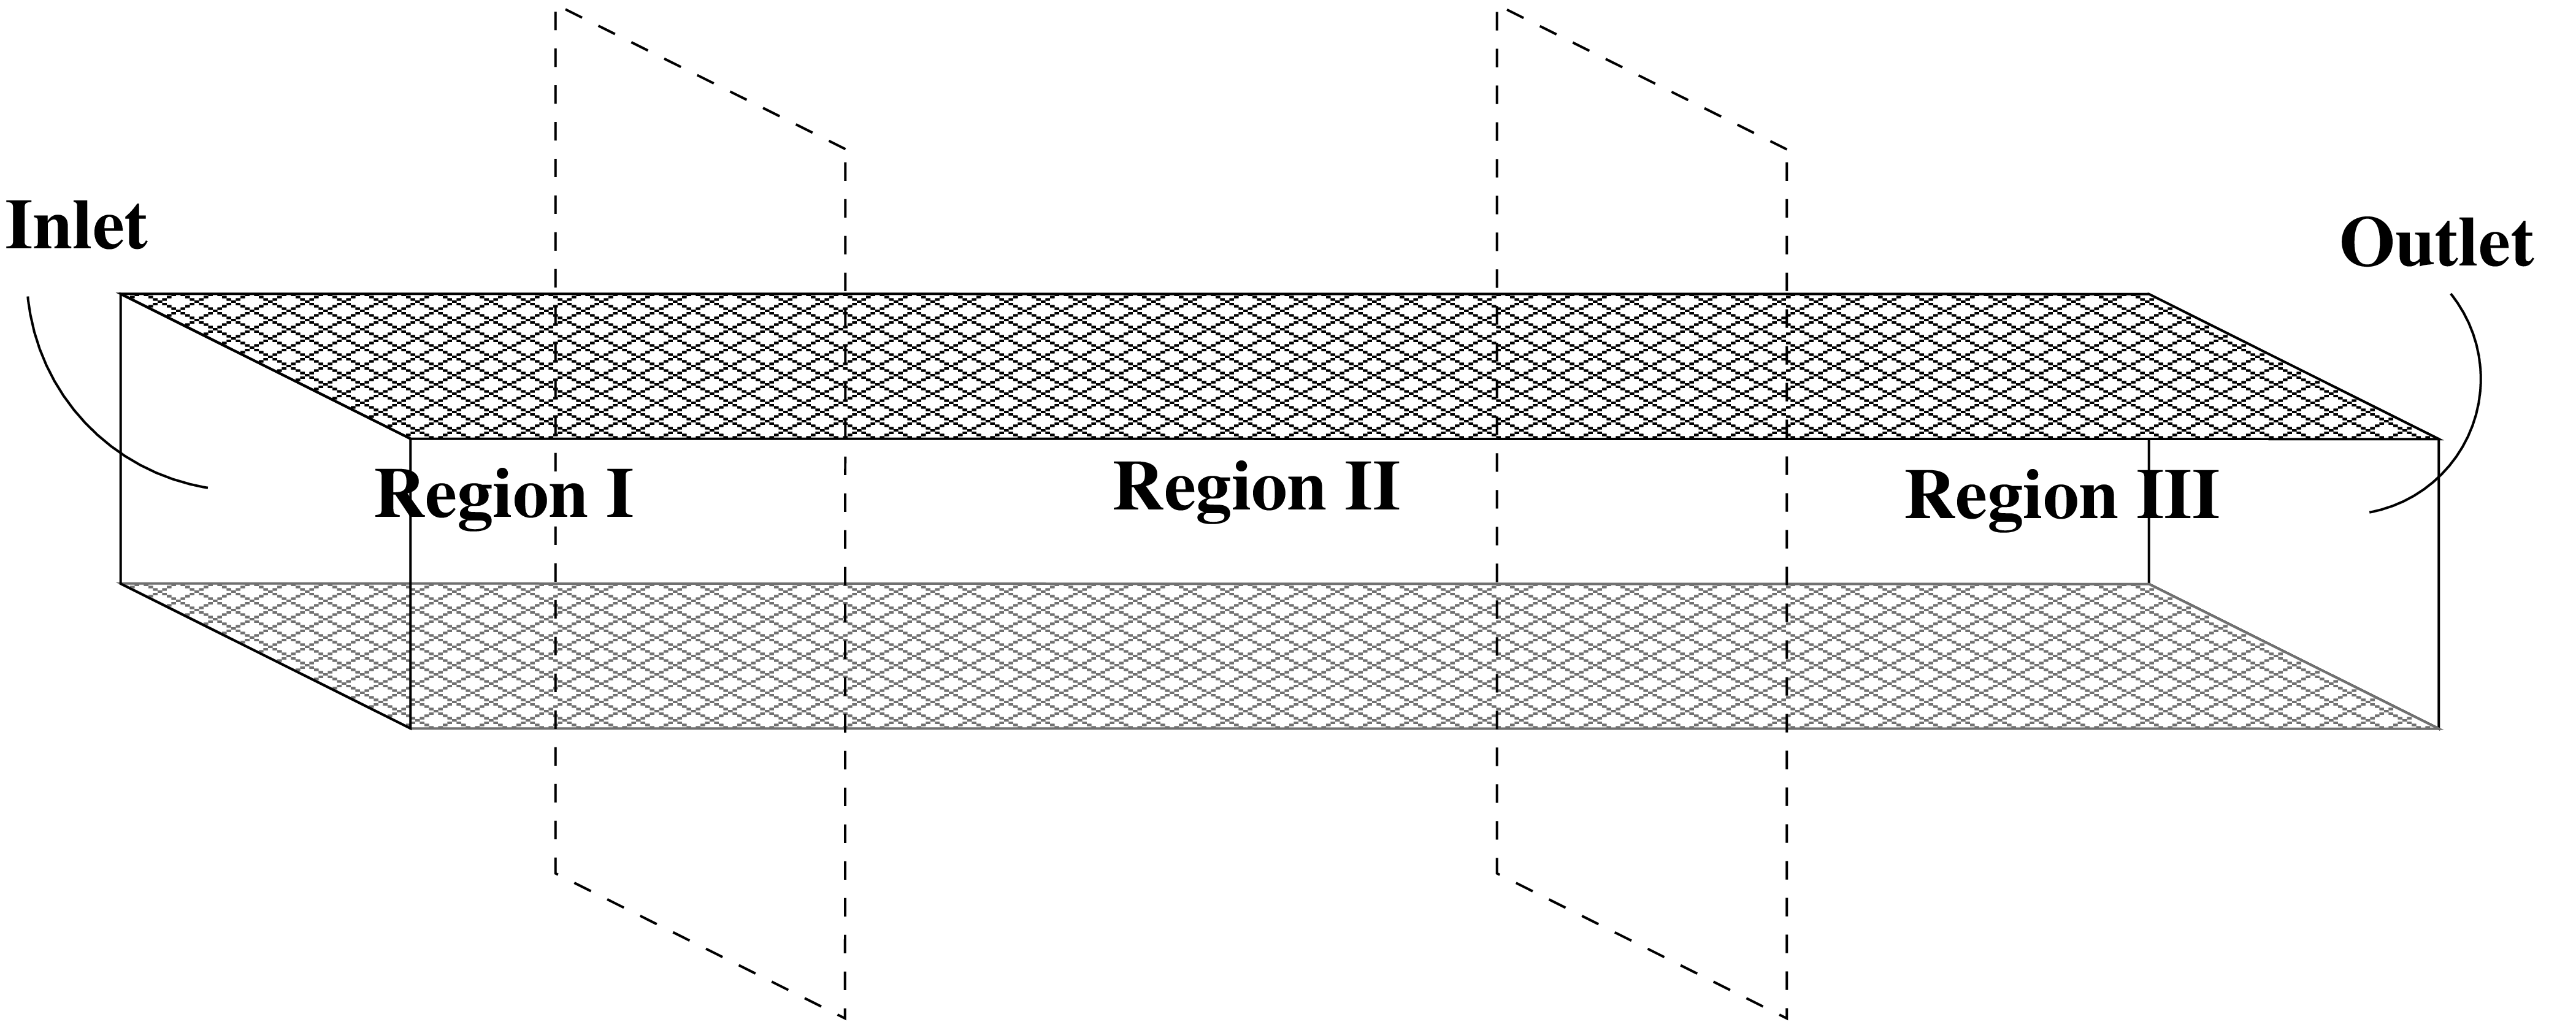
\includegraphics[trim = 20mm 15mm 30mm 10mm, width = 85mm]{turbchannel_a.png}
	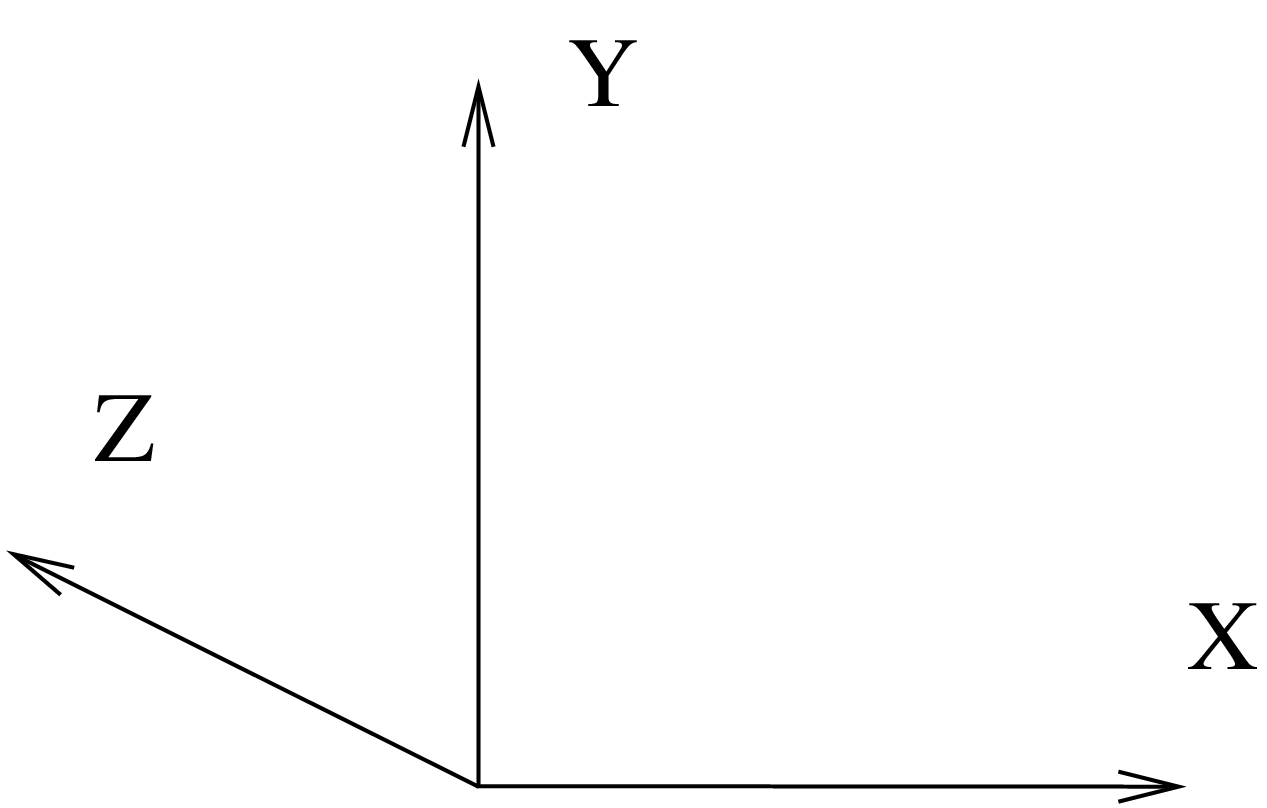
\includegraphics[trim = 0mm 0mm 0mm 20mm, width = 15mm]{axis.png}
	\caption{GEOMETRY OF THE TURBULENCE CHANNEL, THE CHANNEL IS DIVIDED INTO THREE DIFFERENT REGIONS.} % subcaption
	\label{fig:geometries}
	\end{figure}

\begin{figure}[!htbp]
	\centering
	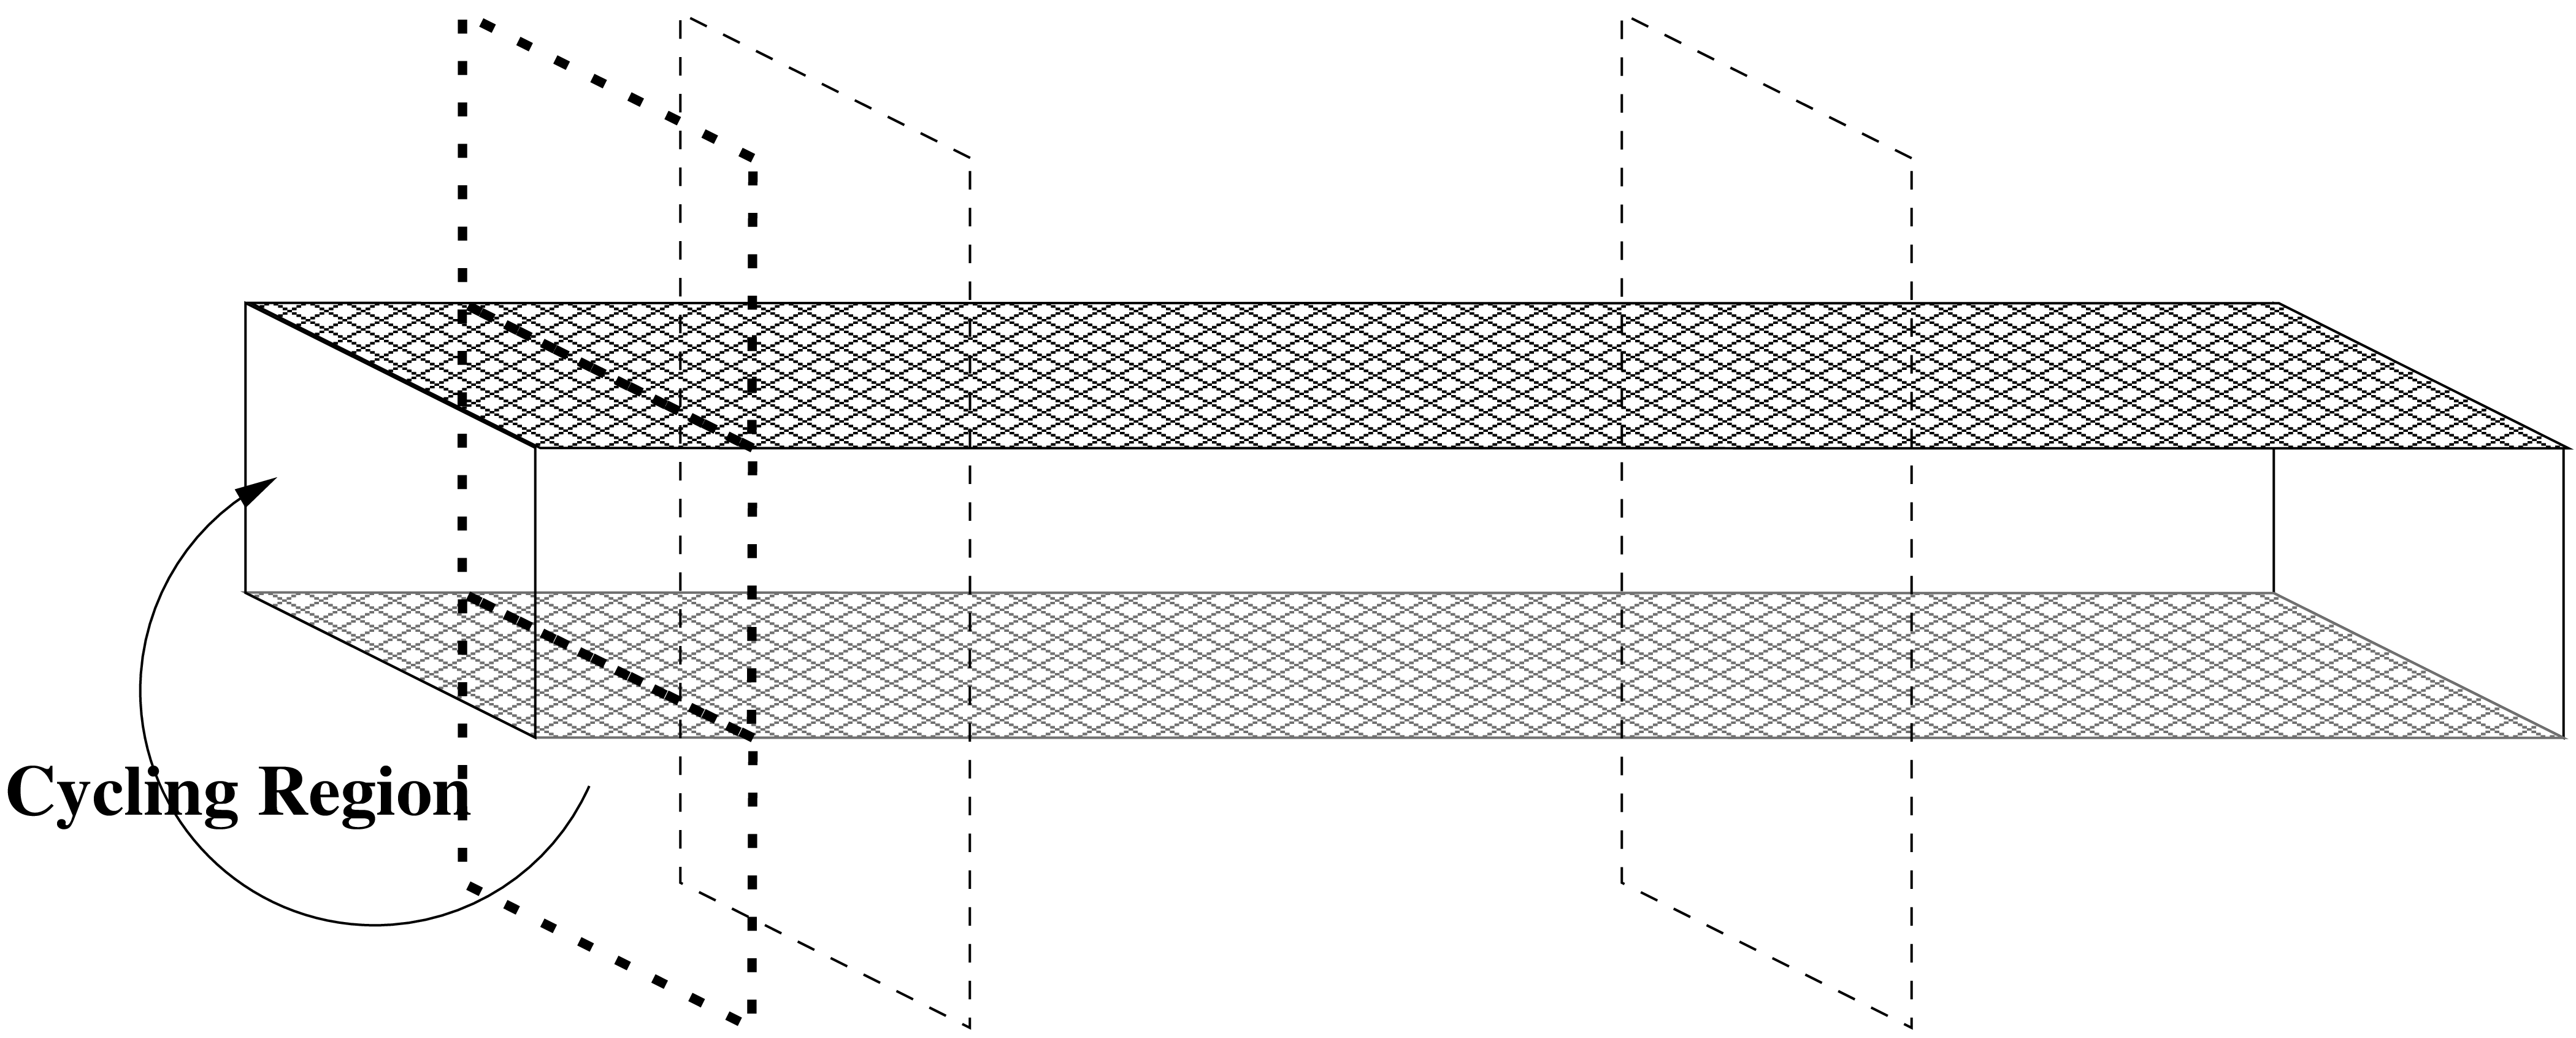
\includegraphics[trim = 20mm 15mm 30mm 10mm, width = 85mm]{turbchannel_b.png}
	\caption{CYCLIC REGION IN THE INLET.} 
	\label{fig:inlet}
\end{figure}

\begin{figure}[!htbp]
	\centering
	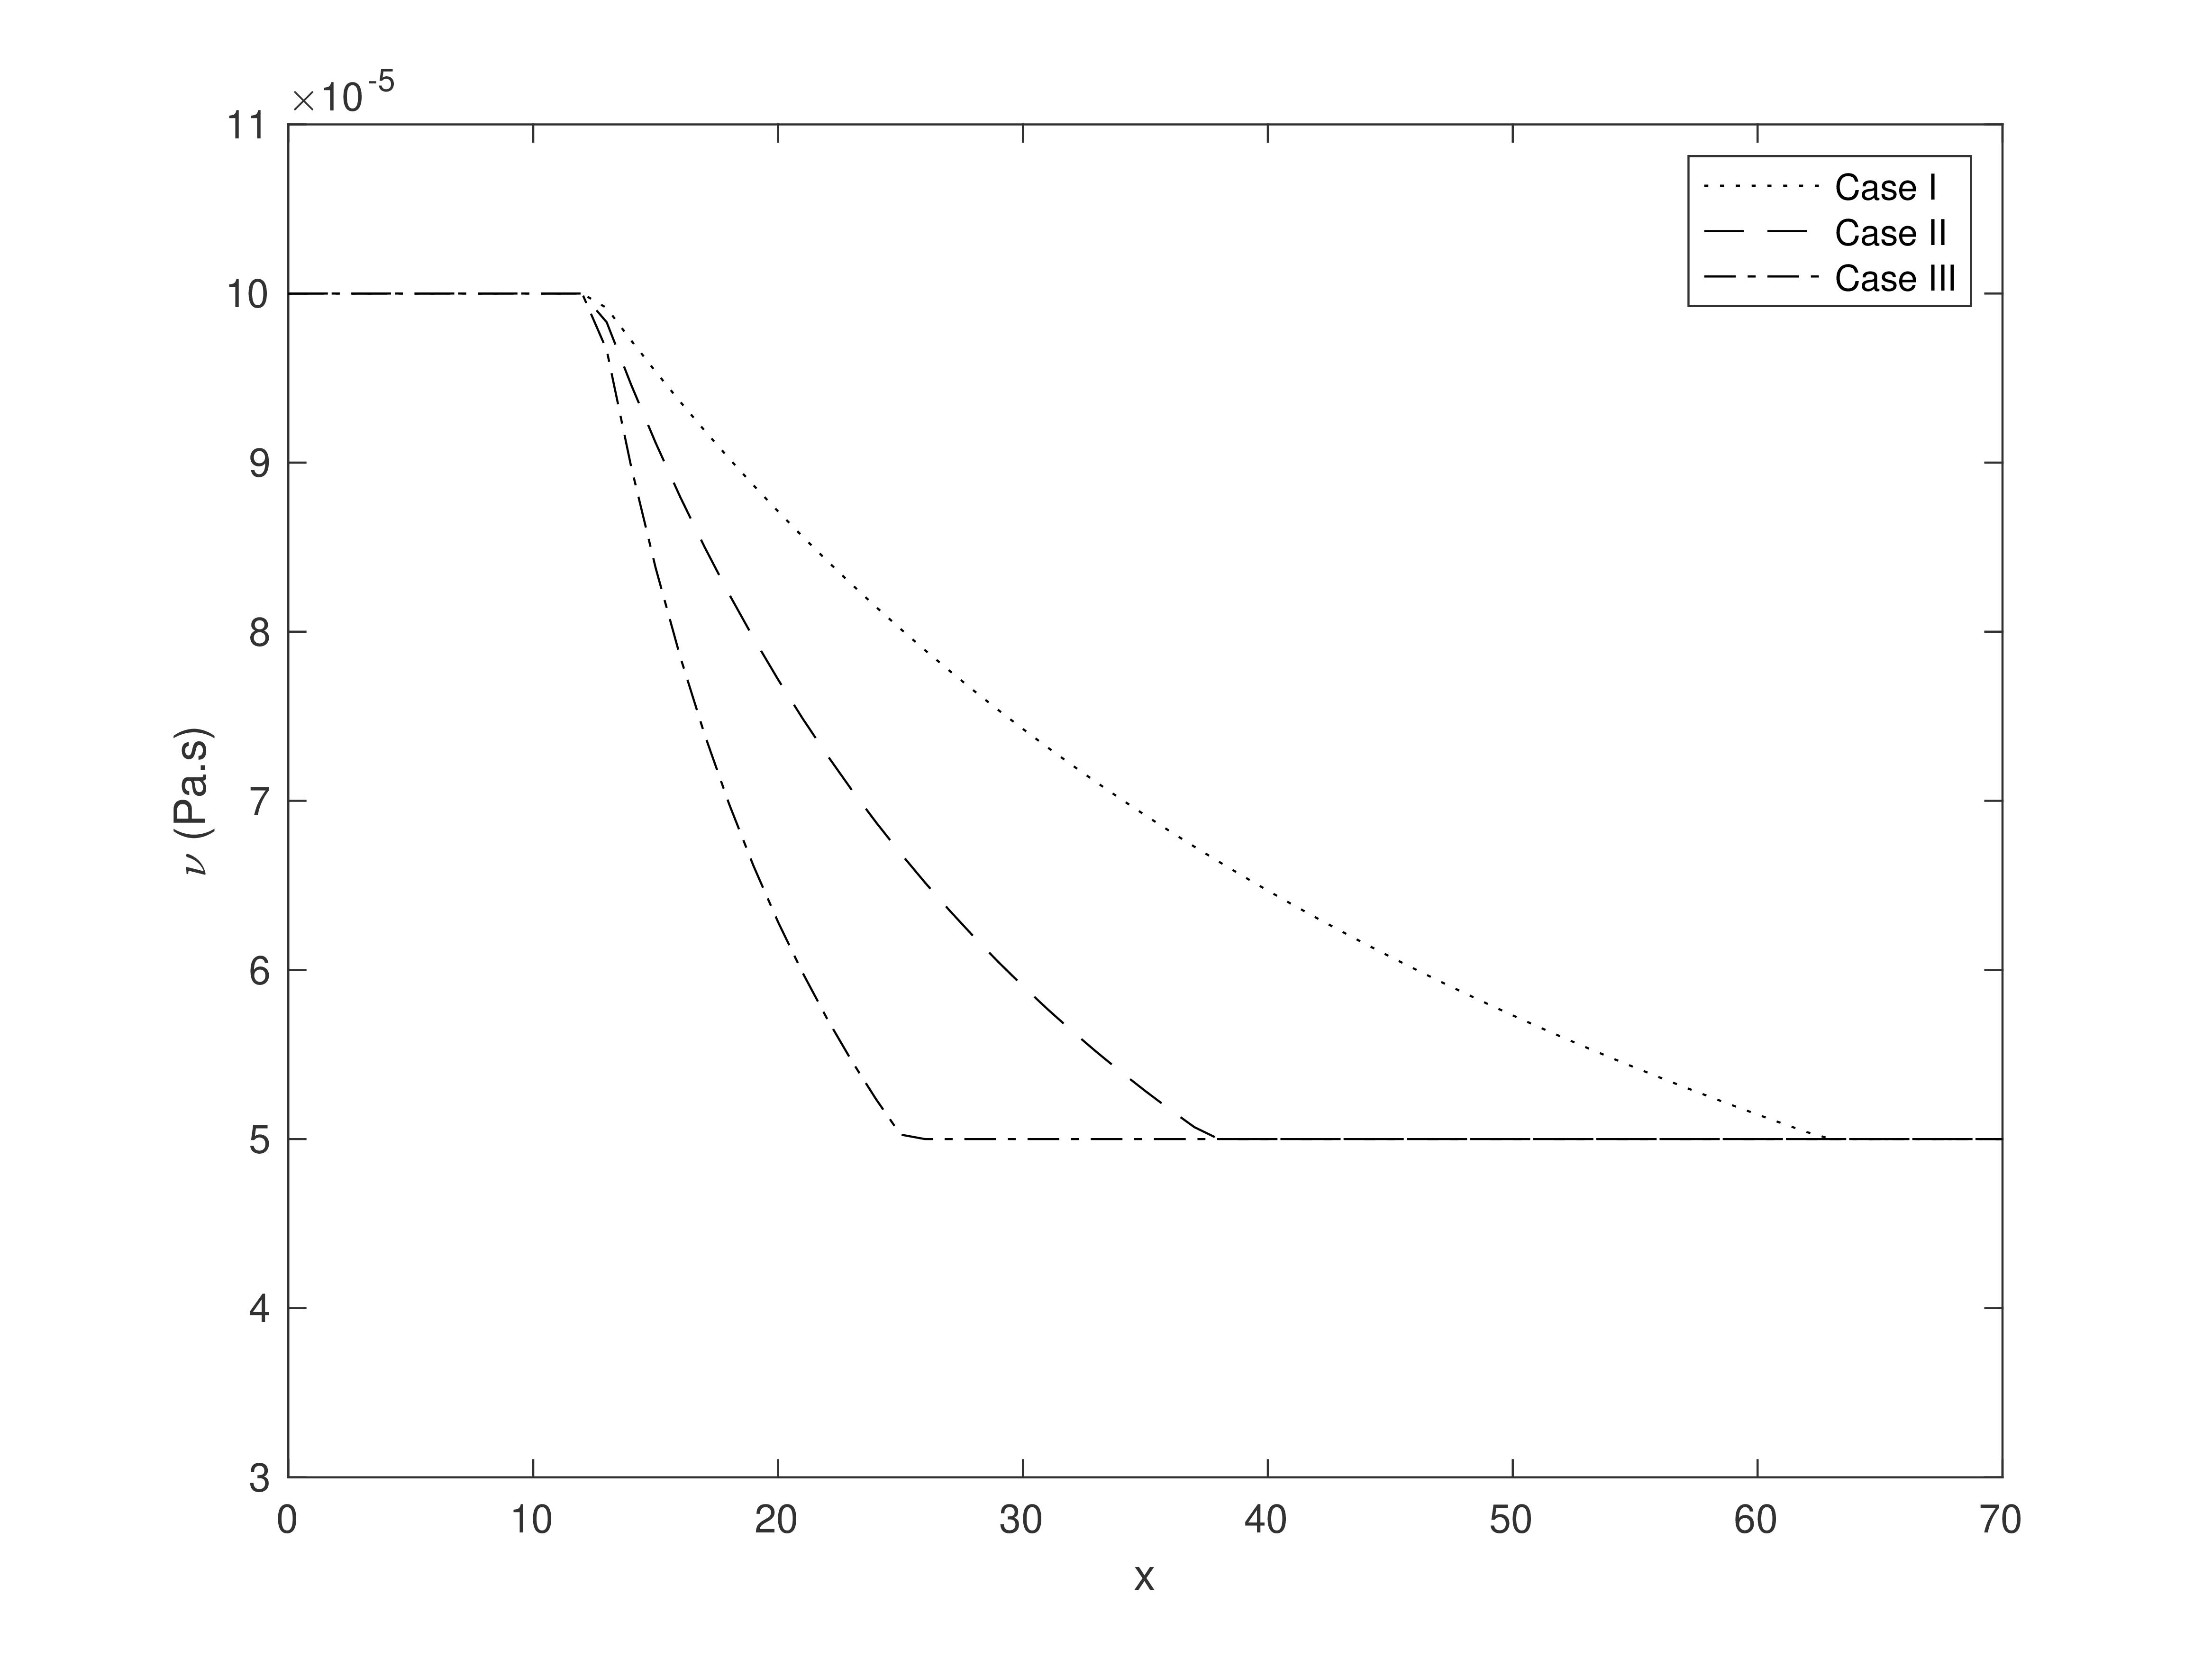
\includegraphics[trim = 20mm 15mm 30mm 10mm, width = 85mm]{viscosity.png}
	\caption{THE VISCOSITY FROM THE THREE CASES VARYING ALONG THE STREAMWISE DIRECTION.}
	\label{fig:viscosity_cases}
	\end{figure}

\begin{figure}[!htbp]
	\centering
	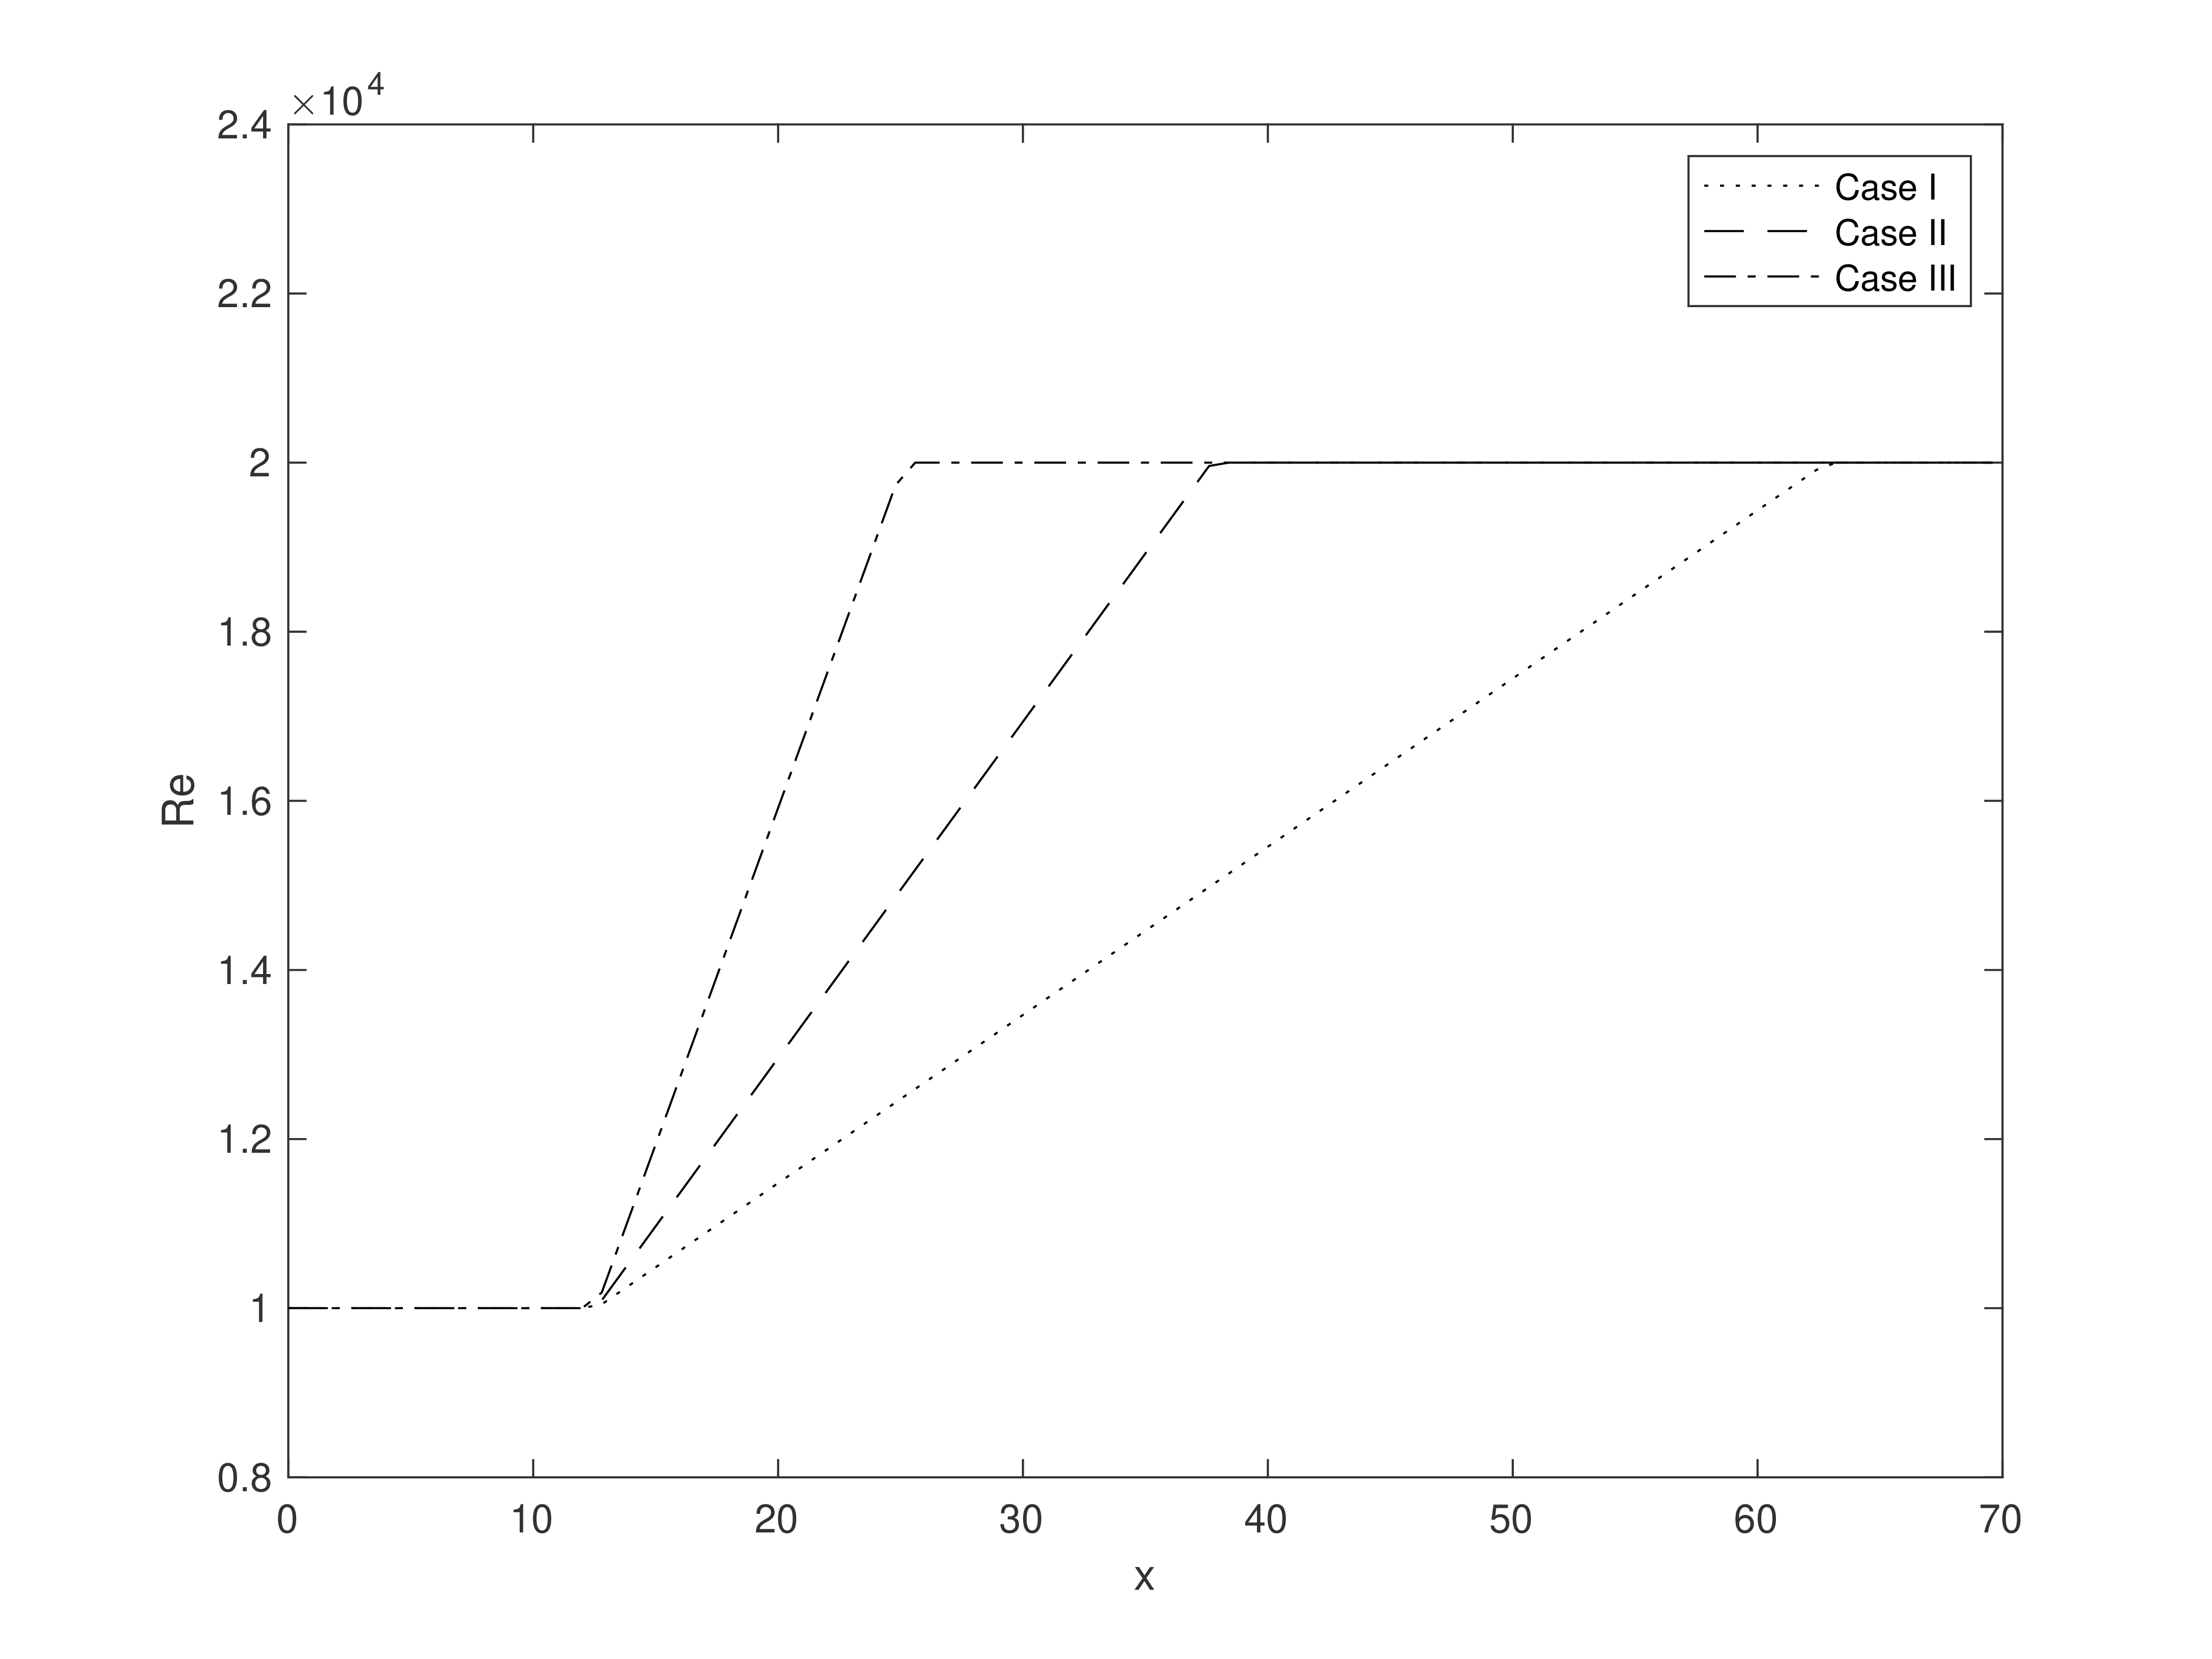
\includegraphics[trim = 20mm 15mm 30mm 10mm, width = 85mm]{Re_across_x.png}
	\caption{THE REYNOLDS NUMBER FROM THE THREE CASES VARYING ALONG THE STREAMWISE DIRECTION.}
	\label{fig:reynolds_n}
\end{figure}

%%%%%%%%%%%%%%%%%%%%%%%%%%%%%%%%%%%%%%%%%%%%%%%%%%%%%%%%%%%%%%%%%%%%%%
\section*{METHODS}

In order to resolve the finest turbulent scales, the calculations of this work has been developed through Direct Numerical Simulation (DNS). To do so, a spectral element code Nek5000 was employed, where this code has been developed in Argonne National aboratory (ANL) and it has been validated in references \cite{merzari2013} and \cite{Obabko2011}.

The solution of this method is given by trigonometric series, in each element a polynomial functions of up to the twelveth degree have been employed to discretize the velocity field. Fig.~\ref{fig:cross_grid} shows an example of the grid from half of the channel's cross section. One should notice that the discretization presented by this particular area is identical through all model's domain and it is only presented half of the cross-section for better visualization of the frame.

\begin{figure}[!htbp]
\begin{center}
\setlength{\unitlength}{0.012500in}%
  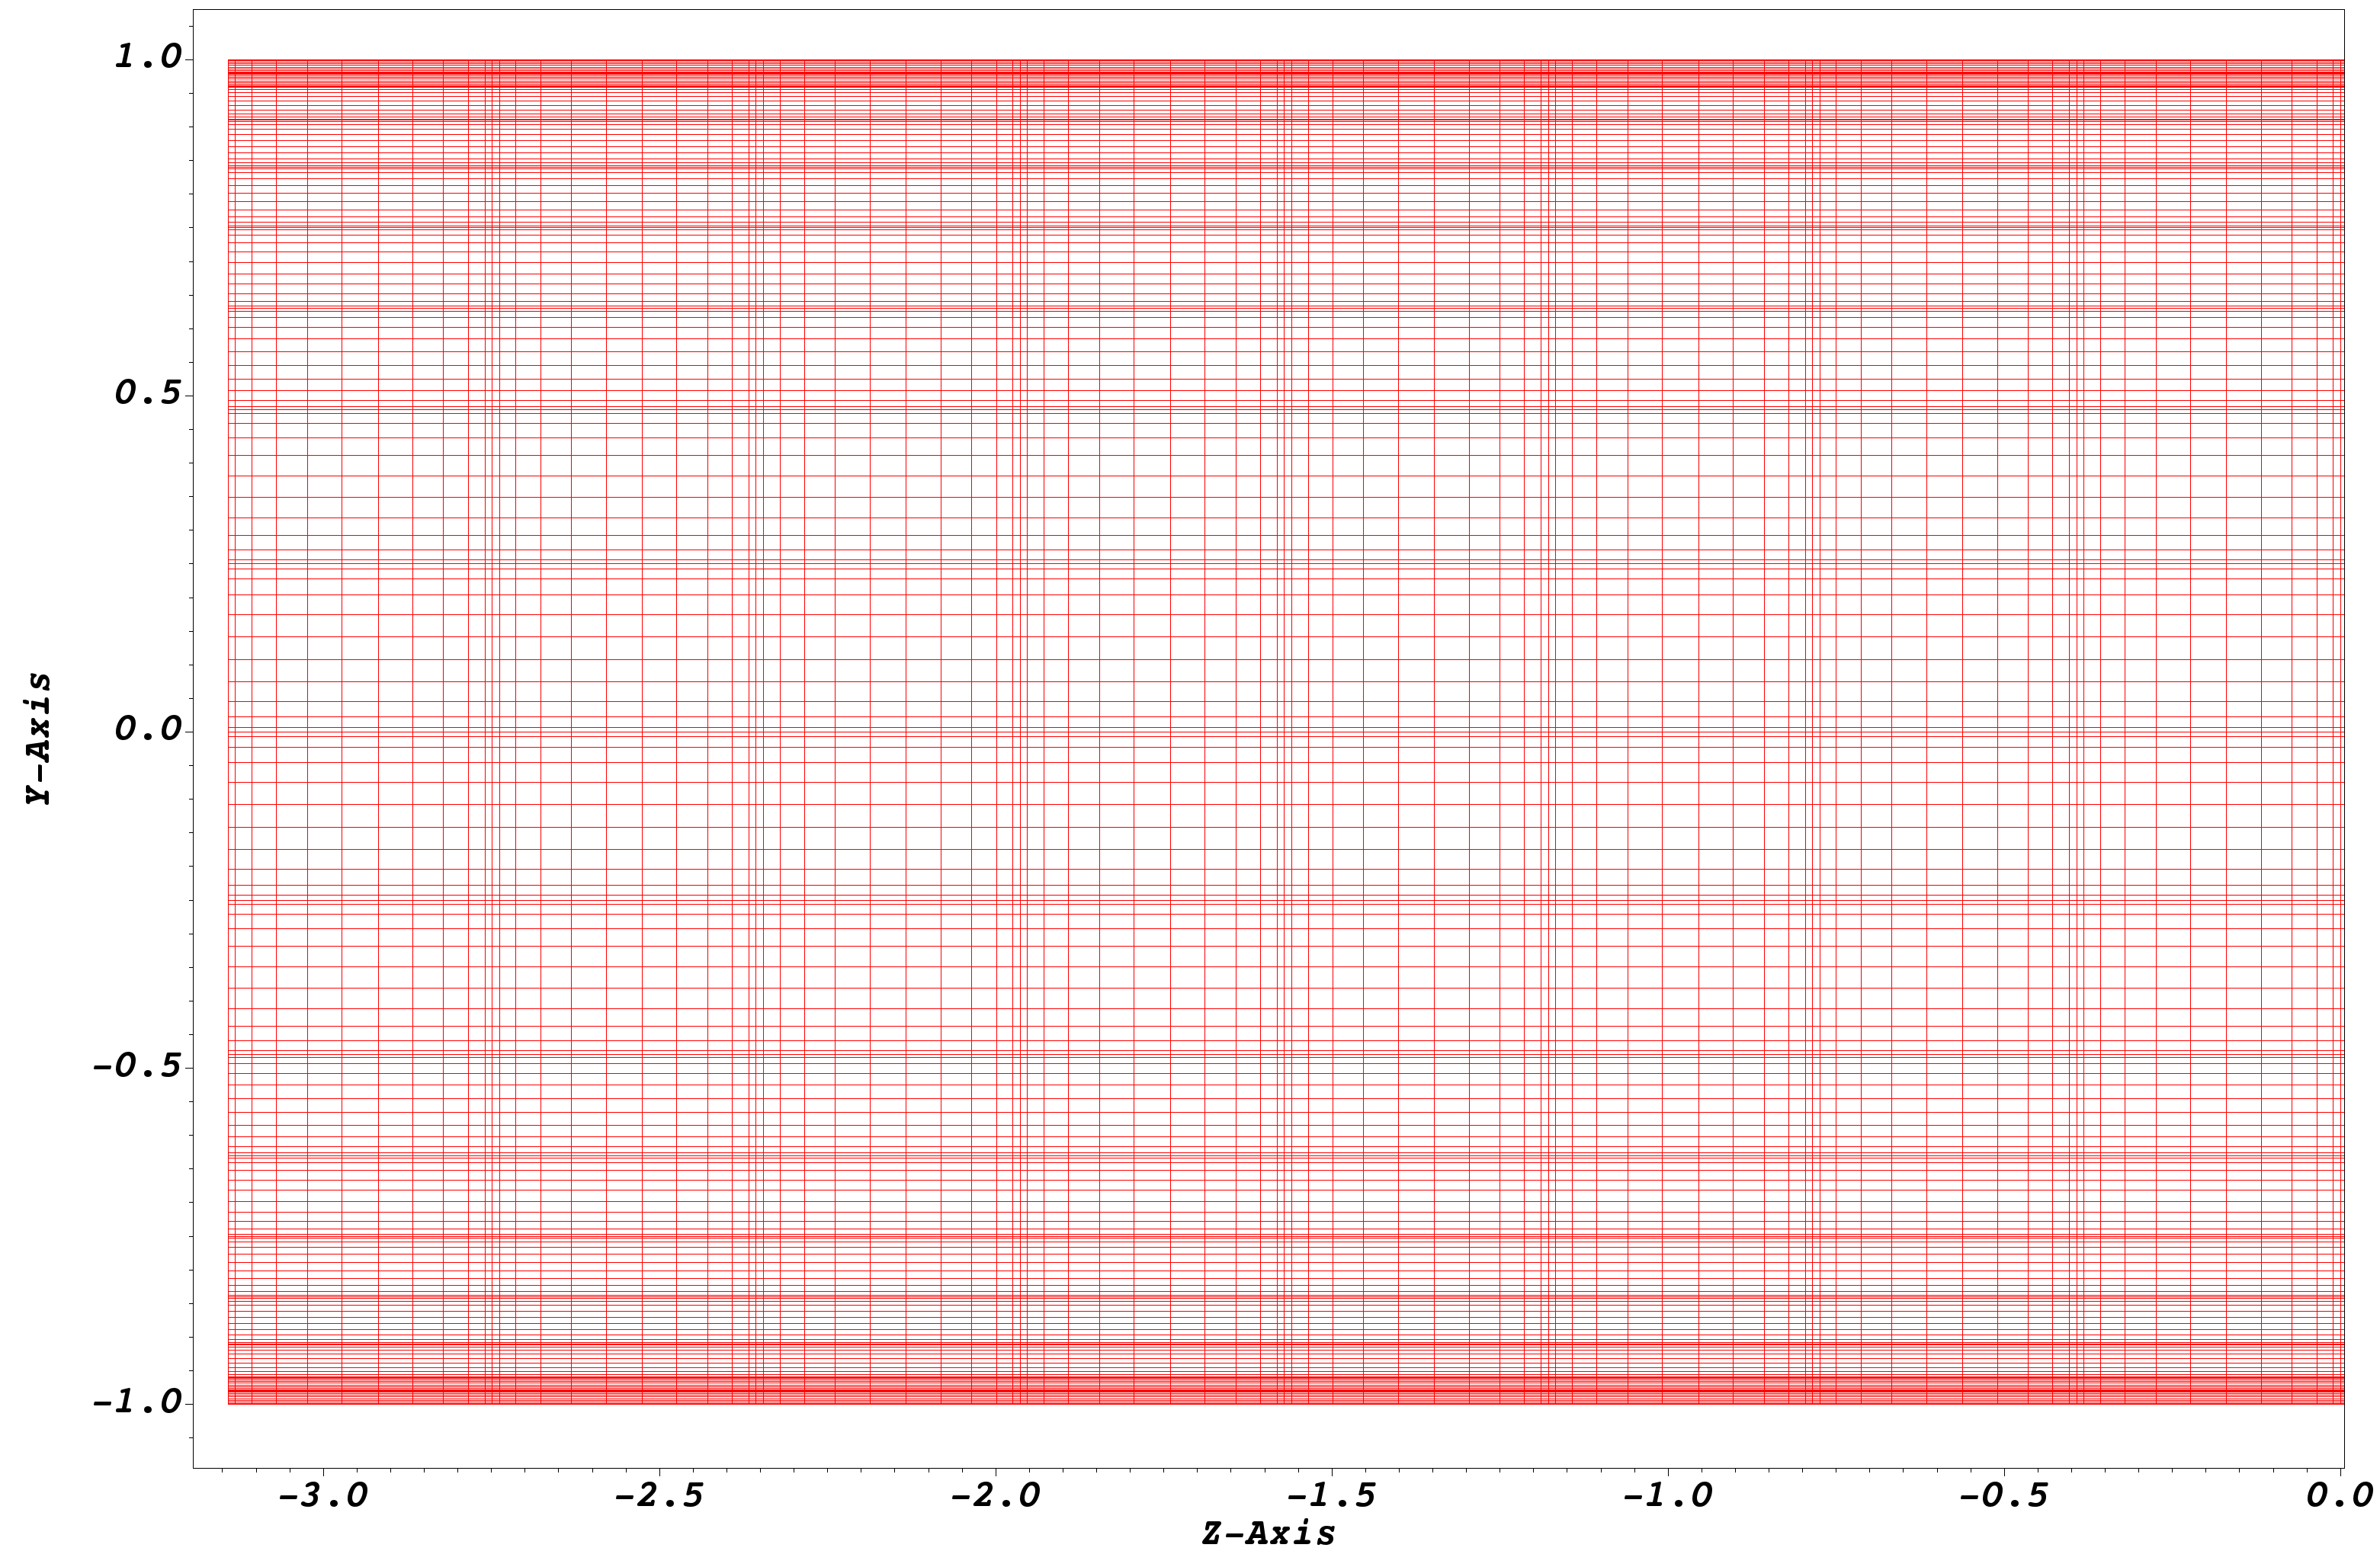
\includegraphics[trim = 20mm 15mm 20mm 10mm, width = 90mm]{half_cross_section_mesh.png}
\end{center}
  \caption{THE GRID EMPLOYED IN THE SIMULATION FROM HALF OF THE CHANNEL'S CROSS SECTION.}
  \label{fig:cross_grid}
\end{figure}

DNS simulations are able to simulate the finest turbulent length scales without using any turbulent model. Since the present work is focused on studying the contribution of the smaller scales to the energy cascade, it is required to use DNS rather than Reynolds Average Navier-Stokes (RANS) or Large Eddy Simulations (LES), although there is a substantial growth of the computational cost.

\underline{Add some stuff about the mesh and polynomial order.}



%%%%%%%%%%%%%%%%%%%%%%%%%%%%%%%%%%%%%%%%%%%%%%%%%%%%%%%%%%%%%%%%%%%%%%

\section*{RESULTS}

The results from the three cases considered in this work are presented in this section. First, the friction Reynolds number variation along the streamwise direction \(x\) of the channels are computed and compared with an expression for \(Re_{\tau}\) as a function of the Reynolds number existed in Ref.~\cite{pope}. This analysis shows the fact that the friction Reynolds number due to a viscosity change imposed through region II is not immediate. Thereon, Reynolds stresses are collected and turbulent structures are investigated along the simulated channels.

%%%%%%%%%%%%%%%%%%%%%%%%%%%%%%%%%%%%%%%%%%%%%%%%%%%%%%%%%%%%%%%%%%%%%%

\subsection*{Analysing the friction Reynolds number}

The friction Reynolds number has been calculated via numerical simulations for Cases I, II and III. To do so, several velocities profiles along \(x\) were obtained from the simulations' results and the viscous stress \(\frac{d\bar{U}}{dy}\) for these locations were calculated. Such values can then be applied in the set of definitions given from Eqn.~\ref{tau_w} to Eqn.~\ref{Re_t} following presented in order to calculate \(Re_{\tau}\).

\begin{equation}
{\tau}_w = \rho\nu\left(\frac{d\bar{U}}{dy}\right)_{y=0}
\label{tau_w}
\end{equation}

Where \(\rho\) is the density and \({\tau}_w\)  is the shear stress at the wall.

\begin{equation}
u_{\tau} = \sqrt{\frac{{\tau}_w}{\rho}}
\label{u_t}
\end{equation}

Where \(u_{\tau}\) is the friction velocity. And finally,

\begin{equation}
Re_{\tau} = \frac{u_{\tau}\delta}{\nu}
\label{Re_t}
\end{equation}

Where \(\delta\) is the height of the simulated channels. For all Cases studied here this is a constant parameter \(\delta=2\).

The friction Reynolds number calculated using Eqn.~\ref{Re_t}, i.e., the numeric simulations' results, are compared to the values obtained using an existed expression in the literature, Eqn.~\ref{anl_ret} from Ref.~\cite{pope}.

\begin{equation}
Re_{\tau} = 0.09Re^{0.88}
\label{anl_ret}
\end{equation}

The Reynolds numbers used to supply Eqn.~\ref{anl_ret} are those varying through \(x\) from Cases I, II and III, as presented in Fig.~\ref{fig:re_t_x}. For simplicity, Reynolds numbers as functions of \(x\) are named in this study as \(Re_{I}(x)\), \(Re_{II}(x)\) and \(Re_{III}(x)\), while the friction Reynolds number functions are named \(Re_{{\tau}I}(x)\), \(Re_{{\tau}II}(x)\) and \(Re_{{\tau}III}(x)\) in reference to their respective cases.

Fig.~\ref{fig:re_t_x} shows the plot of the friction Reynolds number thourgh \(x\) calculated via CFD analisys and by the analytical Eqn.~\ref{anl_ret} for Case I. In this figure, \(Re_{\tau}\) calculated via DNS is delayed in space when compared to the value obtained using the analytical solution provided by Eqn.~\ref{anl_ret}. This fact shows that the effect of the change in the viscosity doesn't cause an immediate effect on the turbulence of the flow. In this sense, the friction Reynolds number calculated through Eqn.~\ref{anl_ret} can be treated as signal over the space \(x\), and a convolution operation can be performed yielding a delayed signal that can be adjusted so it matches to the simulated results. Furthermore, the function \(F_{CI}(x)\) plotted in graph from Fig.~\ref{fig:re_t_x} is the result of this approach, a detailed description about the steps to derive the convolution functions for this study is provided in the following subsection.

\begin{figure}[!htbp]
\begin{center}
\setlength{\unitlength}{0.012500in}%
  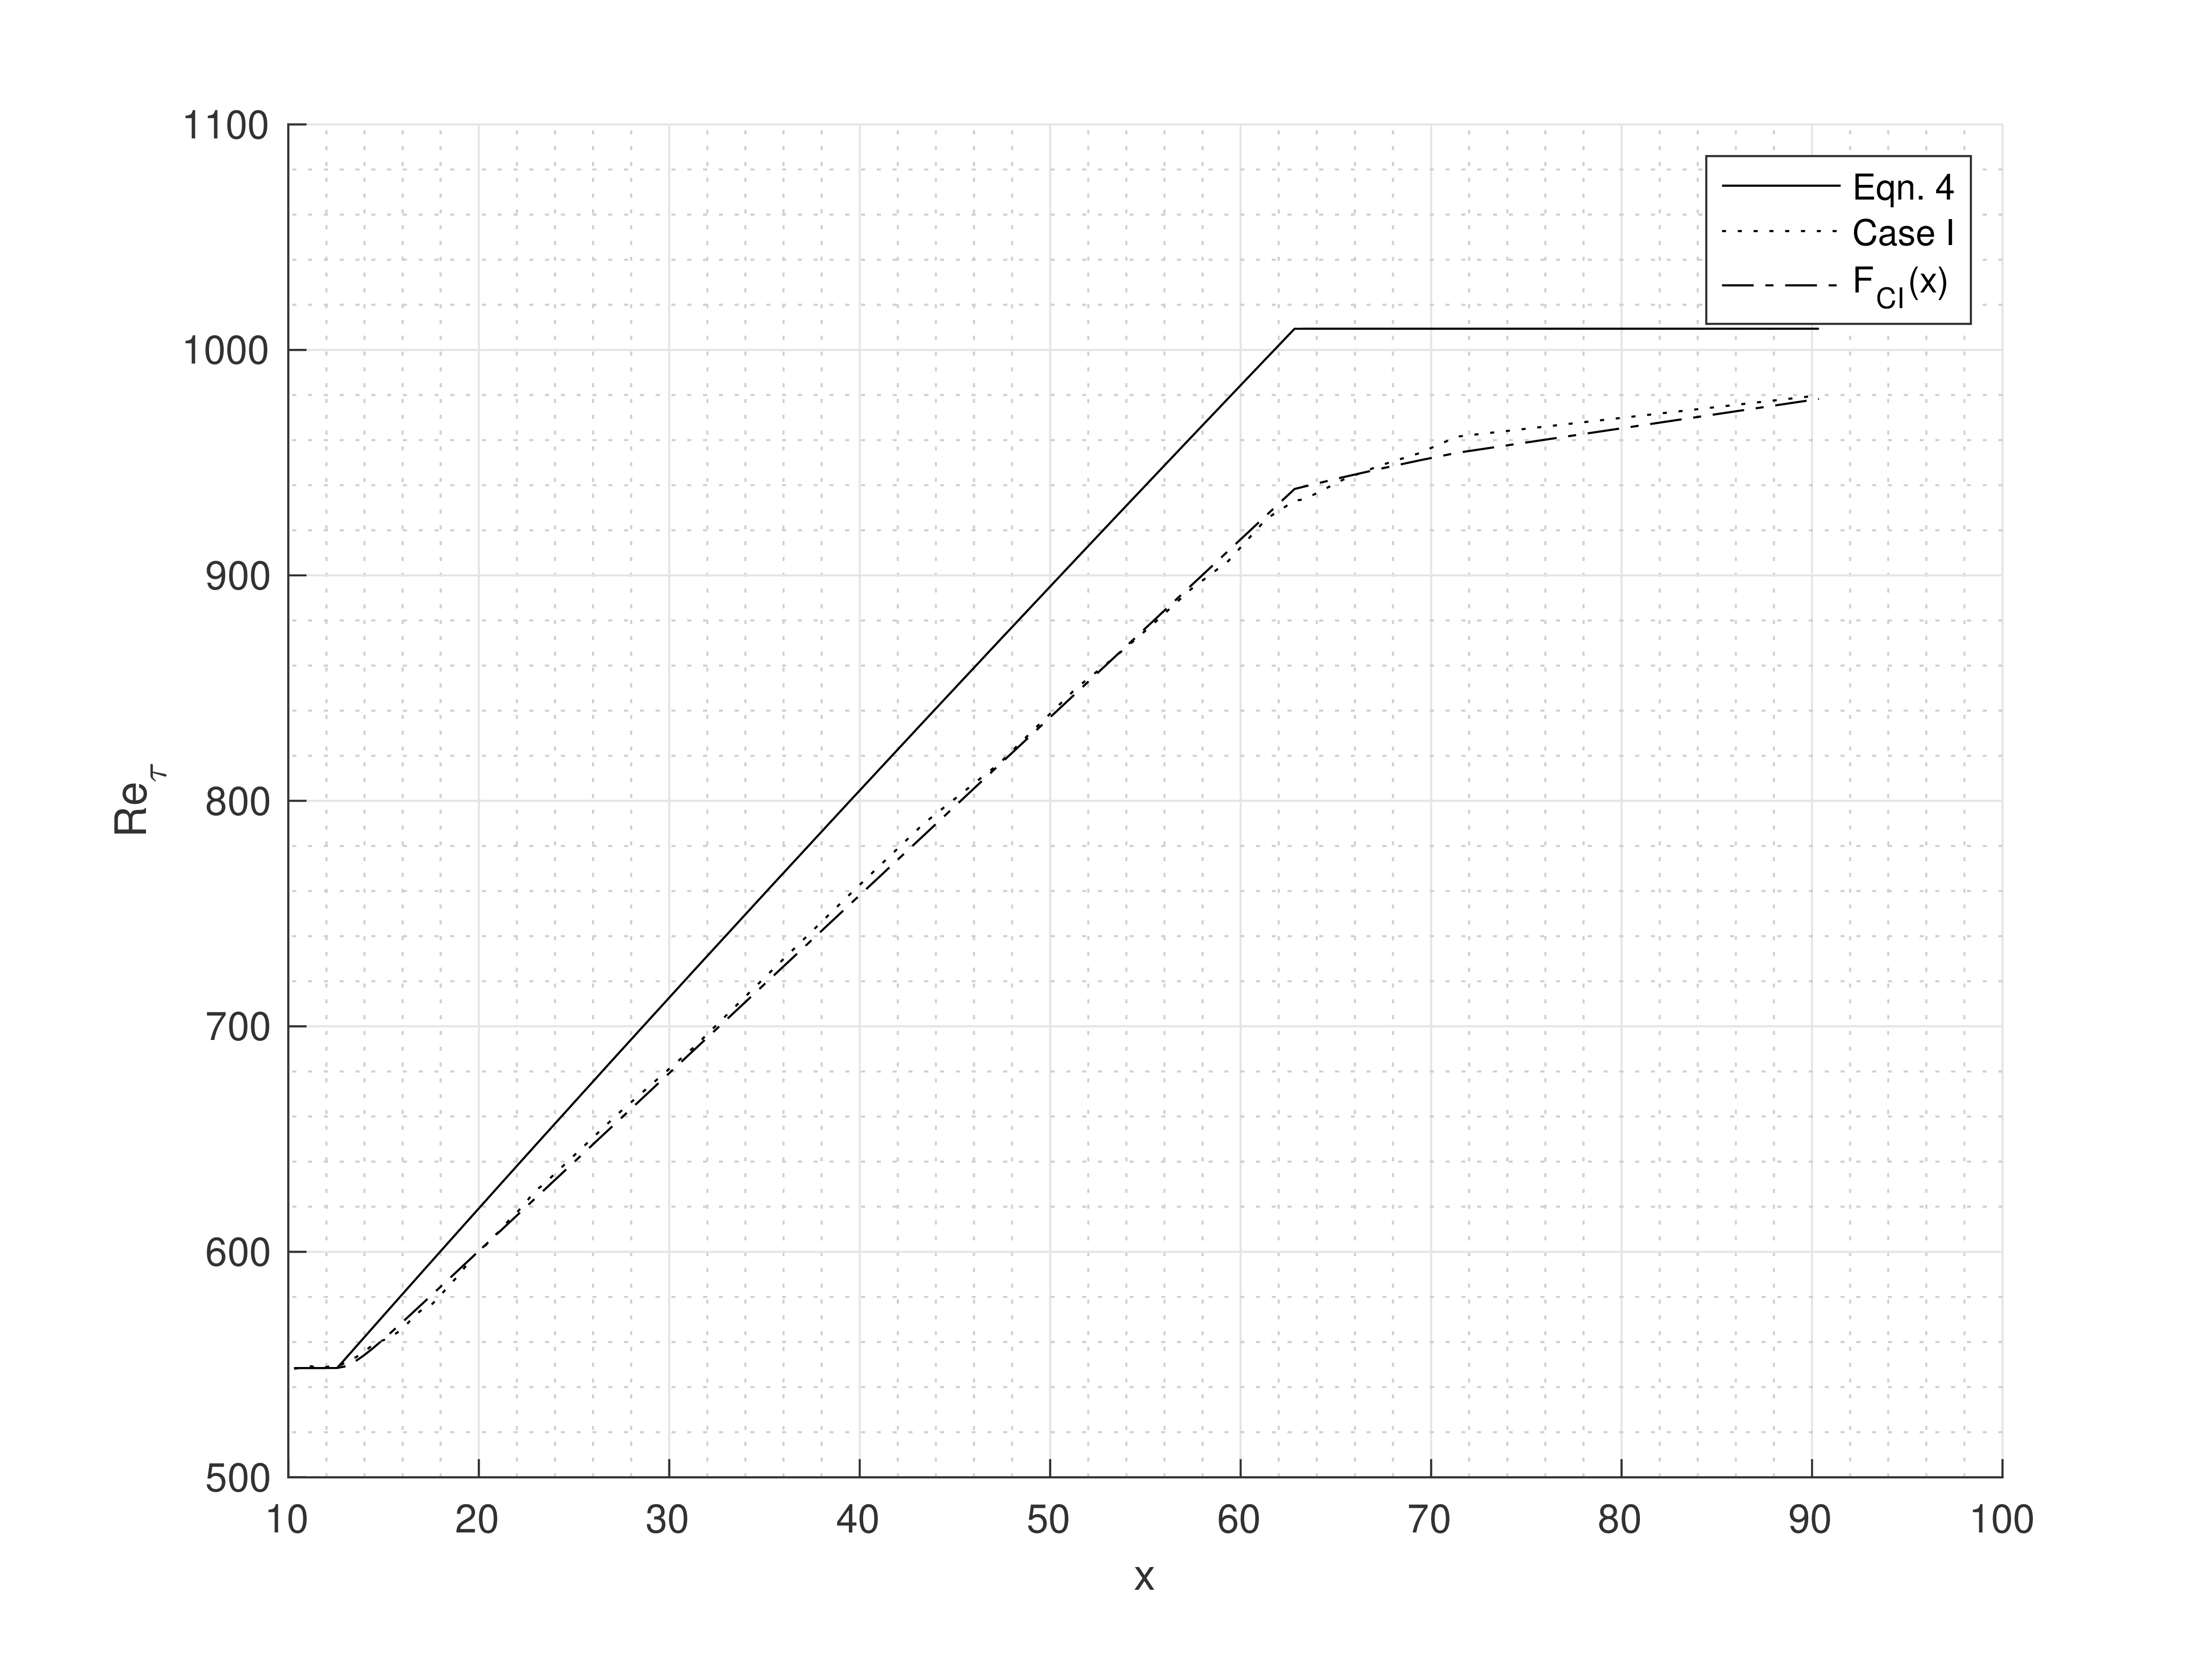
\includegraphics[trim = 20mm 15mm 20mm 10mm, width = 90mm]{Re_t_CI.png}
\end{center}
  \caption{THE FRICTION REYNOLDS NUMBER THOURGH THE STREAMWISE DIRECTION FOR CASE I.}
  \label{fig:re_t_x}
\end{figure}

\subsubsection*{The friction Reynolds number as a delayed signal.} 

The purpose of deriving convolution functions that matches to the simulated data is to have means of quantitativly compute the delay between changing the viscosity and its effect on the turbulence for the studied cases.

Eqn.~\ref{convolution} shows the convolution between the Reynolds number function \(Re(x)\), i.e., one of those presented in Fig.~\ref{fig:reynolds_n}, and a shifting function \(g(x-\chi)\), where \(\chi\) is a dummy variable.

\begin{equation}
F(t) =  \int_{-\infty}^{+\infty} Re_{\tau}(\chi)g(x-\chi)d\chi
\label{convolution}
\end{equation}

Since we are dealing with a delayed signal, a decaying exponential has been used as the shifting function, i.e., \(g(x-\chi)=e^{-Rx}\), like proposed in Ref.~\cite{signals}, where \(R\) is the decaying constant for region II.

The simulated channels in this study are divided in three regions, like shown in Fig.~\ref{fig:geometries}. Since there is no delay in region I, no special treatment is required for it, thus \(F(x)=Re_{\tau}(x)=550\) for \(x{\leq}4\pi\). However, in region II a delay can be seen and a convolution operation needs to be performed for determining a delayed signal. The friction Reynolds number is a linear function given by Eqn.~\ref{linear_ret} in the second region.

\begin{equation}
Re_{\tau}(x)=ax+550
\label{linear_ret}
\end{equation}

Where \(a\) is the linear coefficient that depends on which one of the three cases is being considered. Using Eqn.~\ref{linear_ret} in conjunction to the definition from Eqn.~\ref{convolution}, one may derive Eqn.~\ref{conv_region2}, which is the convolution function valid for region II for the cases considered.

\begin{equation}
F(x)= \frac{a}{R^2}(e^{-R(x-4{\pi})}-1)+\frac{a}{R}(x-4{\pi})+550
\label{conv_region2}
\end{equation}

Lastly, another convolution is performed for region III. However, in this region the signal to be delayed has a constant value, i.e., \(Re_{\tau}(x)=20000\), differing from region II. Because of this, a shifting function with a different decaying constant needs to be considered, thus \(g(x-\chi)=e^{-Cx}\), where \(C\) is the decaying constant for region III. Finally, Eqn.~\ref{conv_region3} can be derived as the convolution function in region III.

\begin{equation}
F(x)= (20000-{\Lambda})(1-e^{-C(x-{\delta}_{R})})+{\Lambda}
\label{conv_region3}
\end{equation}

Where \({\delta}_{R}\) is the \(x\) location of the interface between region II and III depending on which one of the three cases studied is being analysed. Meanwhile, \({\Lambda}=\frac{a}{R^2}(e^{-R({\delta}_{R}-4{\pi})}-1)+\frac{a}{R}({\delta}_{R}-4{\pi})+550\), and it represents the contribution from the predecessors regions.

Tab.~\ref{table_conv} shows the parameters:

\begin{table}[t]
\caption{IMPORTANT PARAMETERS FROM THE CONSIDERED CASES.}
\begin{center}
\centering
\label{table_conv}
\begin{tabular}{c l l l l l}
& & & & \\ % put some space after the caption
\hline
Case	&	Region II length	&	\({\delta}_R\)	&	\(R\)	&	\(C\) \\
\hline
I	&	        \(16{\pi}\)	&	\(20{\pi}\)	&	XXX	&	XXX \\
II	&	        \(8{\pi}\)		&	\(12{\pi}\)	&	XXX	&	XXX \\
III	&	        \(4{\pi}\)		&	\(8{\pi}\)	&	XXX	&	XXX \\
\hline
\end{tabular}
\end{center}
\end{table}

\subsection*{Reynolds stresses and turbulent structures}

More good stuff.




\bibliography{asme2e}
\appendix   

\end{document}
